\documentclass{article}
\usepackage[utf8]{inputenc}
\usepackage{amsmath}
\usepackage{mathtools}
\usepackage{graphicx}
\usepackage{latexsym}
\usepackage{url}
\usepackage{subfig}
\usepackage{hyperref}
\hypersetup{
    colorlinks=true,
    linkcolor=black,
    filecolor=magenta,      
    urlcolor=magenta,
}
\renewcommand*\refname{Bibliografie}
\title{Archer}
\date{Mai 2021}
\begin{document}
\begin{titlepage}
    \begin{center}
    \Large
        Universitatea din Craiova\\
        Facultatea de Automatică, Calculatoare și Electronică\\
        \vspace*{1cm}
         
\includegraphics[scale=0.7]{ace}
        \vspace*{1.5cm}
            
        \Huge{\textbf{Problema arcasilor}\\}
        \vspace{0.3cm}
        \Large
        Inteligenta Artificiala
            
        \vspace{1.5cm}
            
        \Large \textbf{Studentă}: Bucă-Ghebaură Elizabetha Alexandrina
        \\\vspace{0.25cm}
        \Large{\textbf{Specializarea}}: Calculatoare Română\\
        \Large\textbf{Grupa}: CR 2.1A\\
         \Large{\textbf{An}}: II\\
        \vfill
    
        \vspace{0.8cm}
            
        \Large
        Iunie 2021
    \end{center}
\end{titlepage}

\renewcommand*\contentsname{\centering \textcolor{black}{ Introducere cuprins}\\\vspace{1cm} } 
\large \tableofcontents
\vspace{1cm}
\begin{abstract} 
\vspace{0.7cm}
      \large Acest raport este o introducere in obiectivele de dezvoltare a temei de casa la disciplina Inteligenta Artificiala. Documentul contine, de asemenea, o descriere a livrabilelor.
    \end{abstract} 

\newpage
\section{Enuntul problemei}
\vspace{1cm}
\hspace{1cm}Să presupunem grila \textit{k × k} prezentată în Figura 2. Grila este configurată cu un model de pereți. Vi se cere să plasați \textbf{n} arcași pe această grilă astfel încât să nu se poată împușca reciproc. Un arcaș poate trage în sus, în jos, la stânga, la dreapta și, de asemenea, în diagonală, iar împușcătura sa poate ajunge la cel mult \textbf{w} locații în toate direcțiile, până la marginile grilei. \\
\begin{itemize}
\item[a.] Scrieți o formulare detaliată pentru această problemă de căutare. \\
\item[b.] Identificați un algoritm de căutare pentru această sarcină și explicați alegerea dvs.
\end{itemize}
\begin{figure}[htbp!]
\centering
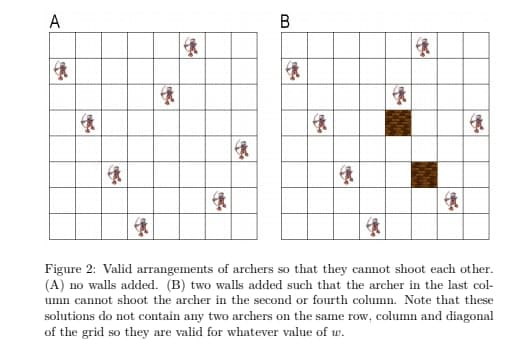
\includegraphics[scale=0.9]{archers}
\end{figure}

\newpage 
\section{Descrierea si intelegerea problemei}
\vspace{0.9cm} 
\hspace{1cm} Aceasta problema este asemanatoare cu cea a reginelor (the eight queens puzzle). \\
\begin{figure}[htbp!]
\centering
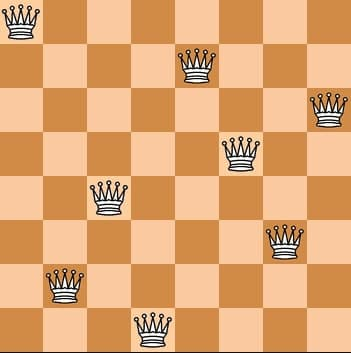
\includegraphics[scale=0.7]{queens}
\end{figure}\\

\hspace{1cm}Problema damelor (sau problema reginelor) tratează plasarea a opt regine de șah pe o tablă de sah \textbf{n × n} astfel încât să nu existe două regine care se amenință reciproc. Astfel, se caută o soluție astfel încât nicio pereche de două regine să nu fie pe același rând, pe aceeași coloană, sau pe aceeași diagonală. \\

\hspace{1cm}Similar, la problema actuala, trebuie sa plasam n arcasi pe o grila \textbf{k × k} astfel incat acestia sa nu se poata impusca reciproc; de asemenea, nu pot fi pe acelasi rand/coloana/diagonala mai multi arcasi, deci nu trebuie sa se suprapuna. Arcasii pot trage cu sageti in toate directiile (ca la problema cu reginele).\\

\hspace{1cm}Personal, am gandit aceasta problema, pe scurt, astfel: sa folosesc algoritmul \textbf{DFS} pentru a vedea pozitia fiecarui arcas pe grila, sa verific apoi daca se suprapun doi sau mai multi arcasi in acelasi loc, lucru care trebuie facut imposibil si sa adaug un perete acolo unde se afla mai multi arcasi pe aceeasi linie/coloana/diagonala.\\
 
\hspace{1cm} \textbf{\underline{Starea initiala}}\\

La inceput avem un tabel gol, de dimensiune \textbf{N = k × k} (in cazul de fata \textit{N} = 4, in problema noastra - codul creat de mine), si un \textbf{pos} care reprezinta pozitiile arcasilor, pozitiile pe care le vom afla pe parcurs. Acesti arcasi pot trage cu arcul in toate directiile; acest fapt va fi rezolvat in stare finala.\\\\

\hspace{1cm} \textbf{\underline{Starea finala}}\\

Dupa ce vom trece prin toate conditiile, si anume acelea in care se afla mai multi arcasi pe aceeasi linie/coloana/diagonala, vom trece peretii acolo unde se intampla aceste conditii, iar in final vom afisa tot tabelul, cu arcasii si zidurile. \\\\


\hspace{1cm} \textbf{\underline{Actiunile arcasilor}}\\

Un arcas poate trage cu arcul in toate directiile, mai exact in sus, jos, stanga, dreapta si diagonala. Dar acesti arcasi nu se pot impusca unul pe celelalt, lucru ce, de asemenea, se va rezolva in starea finala. \\

\vspace{1cm}

\hspace{1cm} Deci, ca un rezumat, problema ne cere sa pozitionam arcasii pe o grila/un tabel \textbf{k × k} astfel incat acestia sa nu traga reciproc in ei (unul in celalalt), iar acolo unde sunt mai multi arcasi pe aceeasi linie/coloana/diagonala, sa se adauge un perete, iar in final sa se afiseze intreg tabelul (matricea/grila), cu toti arcasii si toti peretii.

\newpage 
\section{Algoritmii propusi}
\vspace{1cm} 
\hspace{1cm}Un algoritm folosit este cel de afisare a matricei (grilei/tabelului) \textbf{k × k}. Am adaugat si exceptia din figura urmatoare, in cazul in care apare o eroare si nu se poate deschide fisierul de iesire. \\

\begin{figure}[htbp!]
\centering
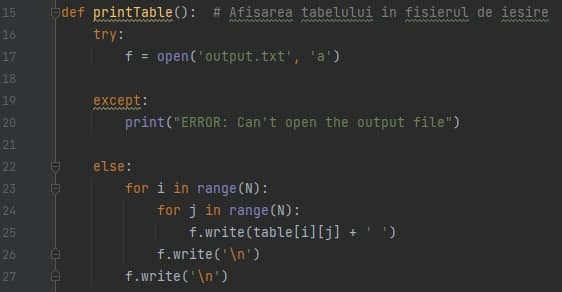
\includegraphics[scale=0.5]{table}
\end{figure}

In pseudocod: \\
\begin{tabbing} 
\indent\textit{func}\={tion}
\textbf{printTable()} \\\\
1. \indent\>\textbf{for} \= i to n \\
2. \indent\>\>\textbf{for} \= j to n \\
3. \indent\>\>end \textbf{for}\\
4. \indent\>end \textbf{for}\\
5. \indent\>{write table[i][j]} \\\\
\indent end \textit{function}\\
\end{tabbing}


Pentru aceasta problema am folosit algoritmul de parcurgere in adancime, si anume \textit{DFS} (\textbf{depth-first search}).  \\

\hspace{0.1cm} Ca o definitie, \textbf{DFS} este un algoritm pentru parcurgerea sau căutarea într-o structură de date de tip arbore sau graf. Se începe de la rădăcină (sau alegând un nod arbitrar ca rădăcină în cazul unui graf) și se explorează cât mai mult posibil de-a lungul fiecărei ramuri înainte de a face pași înapoi. \\

\hspace{0.1cm}In acest caz, rolul cautarii in adancime \textit{DFS} este de a parcurge pozitiile arcasilor. \\\\
\\

\begin{figure}[htbp!]
\centering
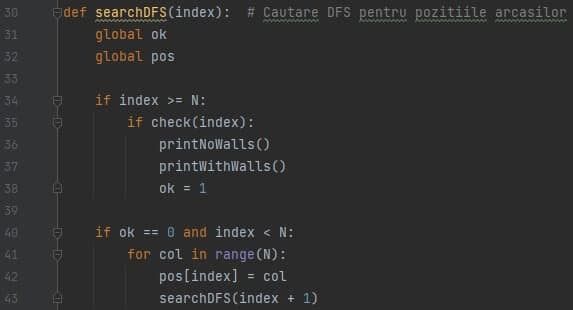
\includegraphics[scale=0.5]{dfs}
\end{figure}

Pentru codul meu, pseudocodul este urmatorul: \\\\

\begin{tabbing} 
\indent\textit{func}\={tion}
\textbf{searchDFS(index)} \\\\
1. \indent\>\textbf{if}  \= index  $\geq$ N \\
2. \indent\>\>\textbf{if}  \= check(index) \\
3. \indent\>\>\>{printNoWalls()} \\
4. \indent\>\>\>{printWithWalls()}\\
5. \indent\>\>\>{ok = 1}\\
6. \indent\>\>end \textbf{if}\\
7. \indent\>end \textbf{if}\\
8. \indent\>\textbf{if}  \= ok = 0 and index $<$ N \textbf{then} \\
9. \indent\>\>\textbf{for}  col to N \\
10. \indent\>\>\>{pos[index] = col} \\
11. \indent\>\>\>{searchDFS(index + 1)} \\
12. \indent\>\>end \textbf{for}  \\
13. \indent\>end \textbf{if}  \\
\indent end \textit{function}
\end{tabbing}

\section{Date experimentale}
\vspace{1cm} 
\hspace{1cm}  Am folosit functia pentru generare automata de date aleatorii randint. Aceasta functie returneaza un numar aleator \textbf{X} astfel incat \textbf{a} $\leq$ \textit{X} $\leq$ \textbf{b}; parametri: (\textbf{start}, \textbf{end}).\\

\hspace{0.6cm}Acest \textbf{start} reprezinta \textit{limita inferioară} - este punctul de plecare de la care se generează întregul aleator, iar acest \textbf{end} reprezinta \textit{limita superioară} - este punctul de oprire până la care metoda ar returna întregul aleator.
\\

\hspace*{0.5cm}  Pentru a putea folosi aceasta functie, a trebuit sa importez modulul random, care oferă acces la diferite funcții utile și una dintre ele fiind capabilă să genereze numere aleatorii, care este \textbf{randint()}.\\ 
\\
\hspace*{1cm}  In programul meu, linia de cod unde este folosita aceasta functie este: \\
\\
$\bullet$ \textbf{\textit{wall\_l = randint(0, N - 1)}} $\rightarrow$ ceea ce inseamna ca va returna un numar intreg aleatoriu astfel incat sa fie cuprins in intervalul (0, N - 1).

\section{Proiectarea aplicației experimentale}
\vspace{0.8cm} 
\subsection{Structura de nivel inalt a aplicatiei}
\hspace{1cm}Aceasta figura reprezinta programul meu cu toate sursele create si anume \textbf{\textit{main.py}} si \textbf{\textit{functions.py}}. \\

\begin{figure}[htbp!]
\centering
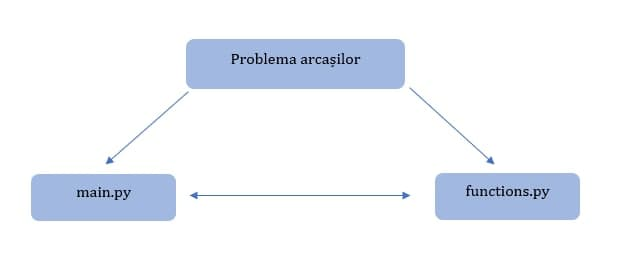
\includegraphics[scale=0.7]{arch}
\end{figure}
In \textbf{\textit{main.py}} sunt apelate functiile problemei, cu timpul de executie, iar in \textbf{\textit{function.py}} sunt implementate toate functiile problemei.
\subsection{Specificarea datelor de intrare}

\hspace{0.5cm}Ca date de intrare am ales cateva variabile de tip intreg si anume: \\\\ 
$\ast$ \textbf{N} - dimensiunea tabelului, care in cazul de fata este 4; \\
$\ast$ \textbf{pos} - pozitiile arcasilor care vor fi aflate pe parcurs; \\
$\ast$ \textbf{wall\_l} - peretele de pe linie, luat aleatoriu; \\
$\ast$ \textbf{wall\_c} - peretele de pe coloana, care de fapt este pozitia peretelui de pe linie. \\

Am ales sa folosesc si cele doua variabile globale si anume \textbf{ok} si \textbf{pos}. Aceste variabile globale pot fi folosite in afara sau in interiorul functiei. \\ 

Functia \textbf{hash()}, in general, dar si in cazul nostru, este folosita pentru a accelera căutările în tabele (de exemplu in bazele de date mari sau comparările de date). \\ 

De asemenea, parcurgerea/cautarea in adancime (\textit{DFS}) a pozitiilor arcasilor a contribuit la specificarea datelor de intrare. \\


\subsection{Specificarea ieșirilor/rezultatelor}

\hspace{0.6cm} In main.py am importat modulul \textbf{timeit} si am folosit functia \textbf{\textit{timeit.default\_timer()}} pentru a "masura" timpul de executie la fiecare  rulare. Practic, biblioteca \textit{Python} (modulul importat) ruleaza codul de foarte multe ori si ofera timpul minim preluat din setul dat de fragment de cod. Aceasta metoda este una utilă, deoarece ajută la verificarea performanței codului. \\\\

\begin{center}
\begin{tabular}{ |p{2.5cm}||p{3cm}|  }
 \hline
 \multicolumn{2}{|c|}{Timpul de executie } \\
 \hline
 0.001670        &  0.003199 \\
 \hline
0.002155       & 0.001857 \\
\hline
0.001358 & 0.003039 \\
\hline
0.021012 & 0.473185 \\
 \hline
\hline
\end{tabular}
\end{center}

\hspace{0cm} Acestui \textbf{\textit{timeit.default\_timer()}} i-am setat valoarea de start si de end, iar la final am afisat diferenta intre acesti doi parametri, adica \textit{end - start} care va rezulta timpul de executie efectuat la fiecare rulare a codului. \\
\\


\begin{figure}%
    \centering
    \subfloat[\centering ]{{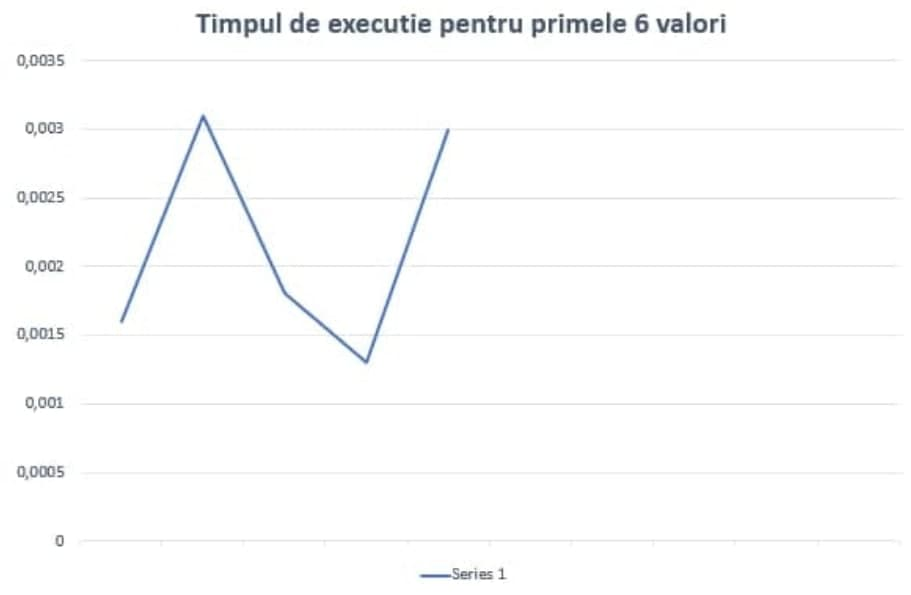
\includegraphics[width=5cm]{grafic1} }}%
    \qquad
    \subfloat[\centering ]{{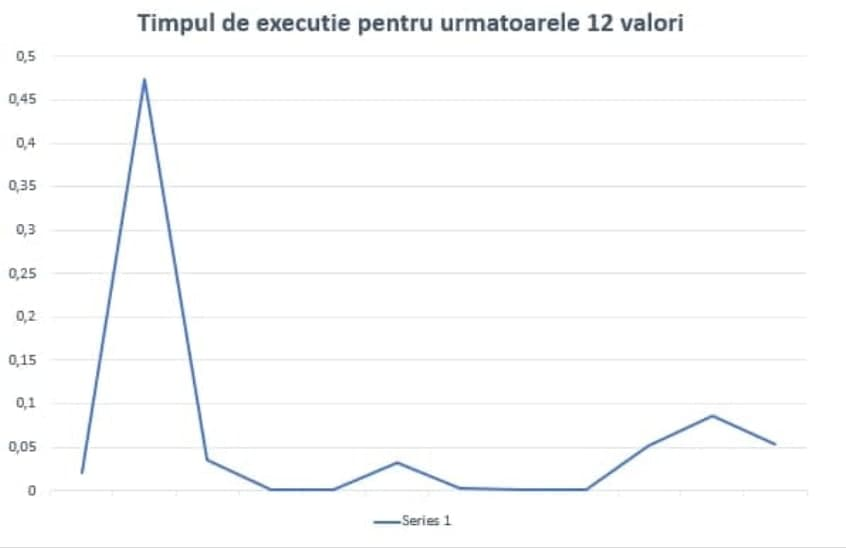
\includegraphics[width=5cm]{grafic2} }}%
    \caption{Graficele timpilor de executie}%
    \label{fig:example}%
\end{figure}

Am atasat mai sus doua exemple de grafice, continand, pe rand, cate 6, respectiv 12 timpi de executie. In aceste grafice se pot observa cresterile si scaderile timpilor de executie, acestia calculati dupa cateva rulari ale codului. \\

Despre datele de iesire mai pot spune faptul ca in cod, spre finalul acestuia, am afisat intreg tabelul cu arcasii si zidurile. Pana sa fac acest lucru, a trebuit sa verific daca arcasul respectiv a putut fi pus in pozitia respectiva si sa pun pereti daca pe aceeasi linie/coloana/diagonala se aflau mai multi arcasi. \\

Acolo unde se pot pozitiona arcasi, in tabelul nostru va aparea litera "\textbf{A}", iar acolo unde vor fi ziduri/pereti, va aparea litera "\textbf{W}" (acestia pusi in functie de pozitia arcasilor - unde se suprapun arcasi, acolo va fi zid intre ei). \\

Deci, in final, pentru datele de iesire vom avea: \\

$\bullet$ \textbf{table[i][pos[i]] = 'A'} - pentru afisarea fiecarui arcas \\

$\bullet$ \textbf{table[wall\_l][wall\_c] = '-'} - pentru afisarea initiala a peretilor; sunt 3 cazuri/conditii atunci cand trebuie sa punem pereti in locul arcasilor care se suprapun: \\

\hspace{1cm} $\bullet$ atunci cand \textbf{n} arcasi sunt plasati pe aceeasi linie, intre ei va fi pus un zid, astfel incat acestia sa nu traga unul in celalalt\\

\hspace{1cm} $\bullet$ atunci cand \textbf{n} arcasi sunt plasati pe aceeasi coloana, intre ei va fi pus un perete, astfel incat sa nu se impuse reciproc \\

\hspace{1cm} $\bullet$ atunci cand \textbf{n} arcasi sunt plasati pe acceasi diagonala, se va introduce un zid intre ei, astfel incat acestia sa nu traga reciproc unul in cealalt \\\\

In cazul de fata, dupa ce se va trece prin fiecare conditie (atunci cand se afla mai multi arcasi pe aceeasi linie/coloana/diagonala), acesti pereti care vor fi pusi intre ei (pentru a nu se impusca intre ei arcasii) vor primi la iesire valoarea de \textbf{"W"}. \\\\
\begin{figure}[htbp!]
\centering
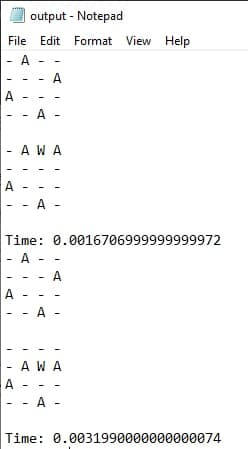
\includegraphics[scale=0.5]{output.jpg}
 \caption{Fisierul de output, dupa rulare}%
\end{figure}

Atunci cand vom rula codul, va aparea, pe rand, la fiecare rulare, tabelul cu arcasii si peretii, precum si timpul de executie. (\textit{Figura 2}) \\


\newpage

\subsection{Lista tuturor modulelor aplicației și descrierea lor}

\hspace{0.5cm} Aici voi realiza o mica prezentare a tuturor modulelor aplicatiei si o descriere a acestora, cu ce scop au fost folosite, de ce si la ce ne ajuta.
Am precizat la subparagraful 5.1 care este structura de nivel inalt a aplicatiei, urmand acum sa specific lista cu toate modulele cat si descierea acestora.\\\\

\hspace{0.5cm} Am ales ca pentru aceasta problema sa folosesc doar doua surse/module si anume cele enumerate mai jos: \\

\begin{itemize}

        \item \textit{\textbf{main.py}} - in acest modul sunt apelate functiile necesare ce se afla în \textsl{functions.py}; aici se calculeaza si timpul de executie a algoritmului, dupa fiecare rulare.
        \item \textit{\textbf{functions.py}} - in acest modul se află multiplele funcții ale programului ce ajută la rezolvarea problemei
\end{itemize}       

\newpage 

\subsection{Lista tuturor funcțiilor aplicației, grupate pe module}
\subsubsection{Descrierea scopului functiei}
\begin{itemize}
        \item \textit{\textbf{main.py}} : 
            
                \hspace*{0.5cm} $\ast$ \textit{timeit.default.timer()} - calculeaza timpul de executie al programului
            
        \item \textit{\textbf{functions.py}} : 
            
                \hspace*{0.5cm} $\ast$ \textit{hash(name)} - am utilizat aceasta functie pentru a accelera cautarea in matrice \\
                \hspace*{0.5cm} $\ast$ \textit{printTable()} - afiseaza tabelul in fisierul de iesire \\
                \hspace*{0.5cm} $\ast$ \textit{searchDFS(index)} - cautarea in adancime pentru pozitiile arcasilor \\
                \hspace*{0.5cm} $\ast$ \textit{check(index)} - verificarea fiecarei pozitii ale arcasului \\
                \hspace*{0.5cm} $\ast$ \textit{threatens(line\_i, col\_i, line\_j, col\_j)} - aici se verifica daca se afla mai multi arcasi pe aceeasi linie/coloana/diagonala \\
                \hspace*{0.5cm} $\ast$ \textit{randomWall()} - functie care returneaza un perete/zid, aleatoriu \\
                \hspace*{0.5cm} $\ast$ \textit{printNoWalls()} - afisarea tabelului cu arcasii, fara pereti \\
                \hspace*{0.5cm} $\ast$ \textit{printWithWalls()} - afisarea tabelului cu arcasii si peretii; aici verificam daca arcasul respectiv poate fi pus in acea pozitie si apoi punem pereti acolo unde sunt arcasi pe aceeasi linie/coloana/diagonala
            
\end{itemize}
\subsubsection{Descrierea fiecarui parametru}
\hspace*{0.5cm} $\ast$ \textit{N} - dimensiunea tabelului NxN \\
\hspace*{0.5cm} $\ast$ \textit{table} - tabelul gol \\ 
\hspace*{0.5cm} $\ast$ \textit{pos} - pozitiile arcasilor \\
\hspace*{0.5cm} $\ast$ \textit{ok/ok1} - contor\\
\hspace*{0.5cm} $\ast$ \textit{index} - numarul arcasului respectiv \\ 
\hspace*{0.5cm} $\ast$ \textit{lin$\_$i $\&$ lin$\_$j} - liniile tabelului in pozitiile i si j \\ 
\hspace*{0.5cm} $\ast$ \textit{col$\_$i $\&$ col$\_$j} - coloanele tabelului in pozitiile i si j \\
\hspace*{0.5cm} $\ast$ \textit{wall$\_$c $\&$ wall$\_$l} - perete de pe coloana/linie 

\subsubsection{Semnificația valorii de return}

$\ast$ \textit{return wall\_l, wall\_c} - returneaza zidurile pe linie si coloana, in mod aleatoriu

\newpage

\section{Concluzii}
\vspace{0.2cm} 
\hspace{0.5cm}$\star$  Observand inca de la inceput ca aceasta problema seamana intr-un oarecare fel cu problema reginelor, am pornit de la acest fapt si cu gandirea asupra modului de rezolvare. \\

$\star$ A fost pentru prima data cand am folosit algoritmul de calculare a timpilor de executie, si mi s-a parut foarte interesant acest lucru: cum sunt de fiecare data acesti timpi diferiti. \\

$\star$ De asemenea, un alt lucru interesant mi s-a parut algoritmul pe care l-am folosit pentru a afla pozitiile arcasilor, si anume cautarea/parcurgerea in adancime, \textit{DFS} . Acesta are o complexitate, la fel ca si parcurgerea in latime, \textit{BFS}, \textbf{O($|$E$|$+$|$V$|$)} (numarul de muchii plus numarul de noduri), care, in cazul cel mai nefavorabil, cand graful/tabelul este liniarizat, vor fi parcurse si explorate toate muchiile si toate nodurile.\\

$\star$ Am ales sa rezolv aceasta problema (denumita de mine problema arcasilor) in limbajul de programare \textbf{Python}, deoarece, avand si anul trecut tema de casa in acest limbaj, mi s-a parut din nou un "challenge" si am dorit sa invat si mai multe despre el. Acest limbaj mi se pare intr-o oarecare masura mai "usor", prin simplul fapt ca este un limbaj de programare interpretat, mai exact ceea ce imi "surade" mie este ca nu mai trebuie sa implementam unele metode(\textit{random}, \textit{timeit}), ci doar le importam, iar \textbf{Python} isi face singur treaba; de asemenea, numele variabilelor nu are semnificatie sau concept pentru un tip de date, acestea fiind de fapt referiri la obiecte. Majoritatea limbajelor compilate/moderne necesita declararea unei variabile, inainte ca aceasta sa poata fi utilizata, iar cum \textbf{Python} este un limbaj interpretat, declararea variabilelor este optionala. \\ 

$\star$ Pe viitor, voi incerca sa imi imbunatatesc experienta si performantele in acest limbaj de programare, \textbf{Python}, dar si in limbajele de programare actuale cunoscute, anume \textbf{C}, \textbf{C++}, \textbf{Java} si \textbf{C$\#$} care, de asemenea, sunt foarte diferite intre ele, ceea ce le face foarte interesante, cel putin din perspectiva mea; ceea ce ma face sa fiu si mai curioasa in ceea ce le priveste.

%  nu mai trebuie nici sa declaram fiecare variabila (de tip int, float, double) deoarece, cum am scris si mai sus, Python este un limbaj interpretat, iar el "stie" cum trebuie sa fie o variabila, fara sa ii spunem noi ce vrem sa fie.


\newpage 
\section{Referinte bibliografice}
\vspace{1cm} 
\begin{thebibliography}{9}

\bibitem{latex}
      \LaTeX~project site \\
      $\bullet$ \url{https://www.overleaf.com/learn/how-to/Creating_a_document_in_Overleaf} \\
      $\bullet$ \url{https://www.caam.rice.edu/~heinken/latex/symbols.pdf}
\bibitem{cormen-latex}
      Python, \url{https://www.w3schools.com/python/default.asp}
\bibitem{latex}
       DFS, \url{https://en.wikipedia.org/wiki/Depth-first_search}
\bibitem{latex}
      Generarea random a numerelor \\ 
       $\bullet$ \url{https://docs.python.org/3/library/random.html}\\
       $\bullet$ \url{https://www.geeksforgeeks.org/python-randint-function/}
\bibitem{latex}
      Timpul de executie,
      \url{https://docs.python.org/3/library/timeit.html}
\bibitem{latex}
      Problema Reginelor - N Queen Problem, \url{https://www.geeksforgeeks.org/n-queen-problem-backtracking-3/}
\bibitem{latex}
     Artificial Intelligence: A Modern Approach,
     \url{http://aima.cs.berkeley.edu/}
      
\end{thebibliography}
\end{document}
